\chapter{Fejlesztői dokumentáció}
\label{ch:impl}

\section{Algoritmus bemutatása}

\begin{definition}
    Egy ponthalmaz egy elemének a Voronoj-cellája a sík egy olyan régiója, amiben minden pont a ponthalmazból a cellához tartozó ponthoz van legközelebb.
\end{definition}

\begin{definition}
    A Voronoj-diagram a sík egy olyan felosztása amiben egy ponthalmaz minden eleméhez egy Voronoj-cellát rendelünk.
\end{definition}

A szakdolgozat keretein belül egy olyan algoritmus került implementálásra, ami egy kétdimenziós sokszöget feloszt Voronoj-cellákra, a magas szintű lépései az \ref{alg:algorithm}. algoritmus pszeudokódban láthatóak. Az algoritmus egy \textit{N} csúcsú alakzat esetén \textit{N} él- és \textit{N} csúcs régióra osztja fel a síkot, amivel azt teljesen lefedi. Mivel a megadott alakzat több egymásban elhelyezkedő poligonból is állhatnak, ezért az algoritmus futása előtt a pontok átrendezésre kerülnek, mert a megadási sorrend alapján kerül megállapításra a távolság előjele. A régiók véges csúcsszámú konvex poligonokkal vannak ábárzolva. Egy régiót úgy határozunk meg, hogy a kezdetben végtelenül nagy korlátokat vágásokkal az adott régióhoz tartozó Voronoj-cella korlátaihoz igazítjuk.

\begin{algorithm}[H]
    \caption{A vágásokat végző algoritmus pszeudokódja}
    \label{alg:algorithm}
    \textbf{Bemenet:} \textit{Shape shape} \\
    \textbf{Kimenet:} \textit{VertexRegion vertexRegions[M], EdgeRegion edgeRegions[M]}\\A meghatározott régióhatárok, M az alakzatban lévő csúcspontok száma.
    \begin{algorithmic}[1]
        \State reoderVertices(\textit{shape})
        \For{$outline$ : $shape$.getOutlines()}
            \For{$i$ : 0$,\ldots,outline$.size() - 1}
                \State $edge1$ = $outline$[i]
                \State $edge2$ = $outline$[(i + 1) \textbf{mod} $outline$.size()]
                \State $vertexRegion$ = initVertexRegion($edge1$, $edge2$)
                \State $vertexRegions$.add($vertexRegion$)
                \State $edgeRegion$ = initEdgeRegion($edge1$)
                \State $edgeRegions$.add($edgeRegion$)
            \EndFor
        \EndFor
        \State $vertexRegions$.cutWithVertices($vertexRegions$)
        \State $vertexRegions$.cutWithEdges($edgeRegions$)
        \State $edgeRegions$.cutWithVertices($vertexRegions$)
        \State $edgeRegions$.cutWithEdges($edgeRegions$)
        \State \textbf{return} \textit{\{vertexRegions, edgeRegions\}}
    \end{algorithmic}
\end{algorithm}

\begin{figure}[H]
    \centering
    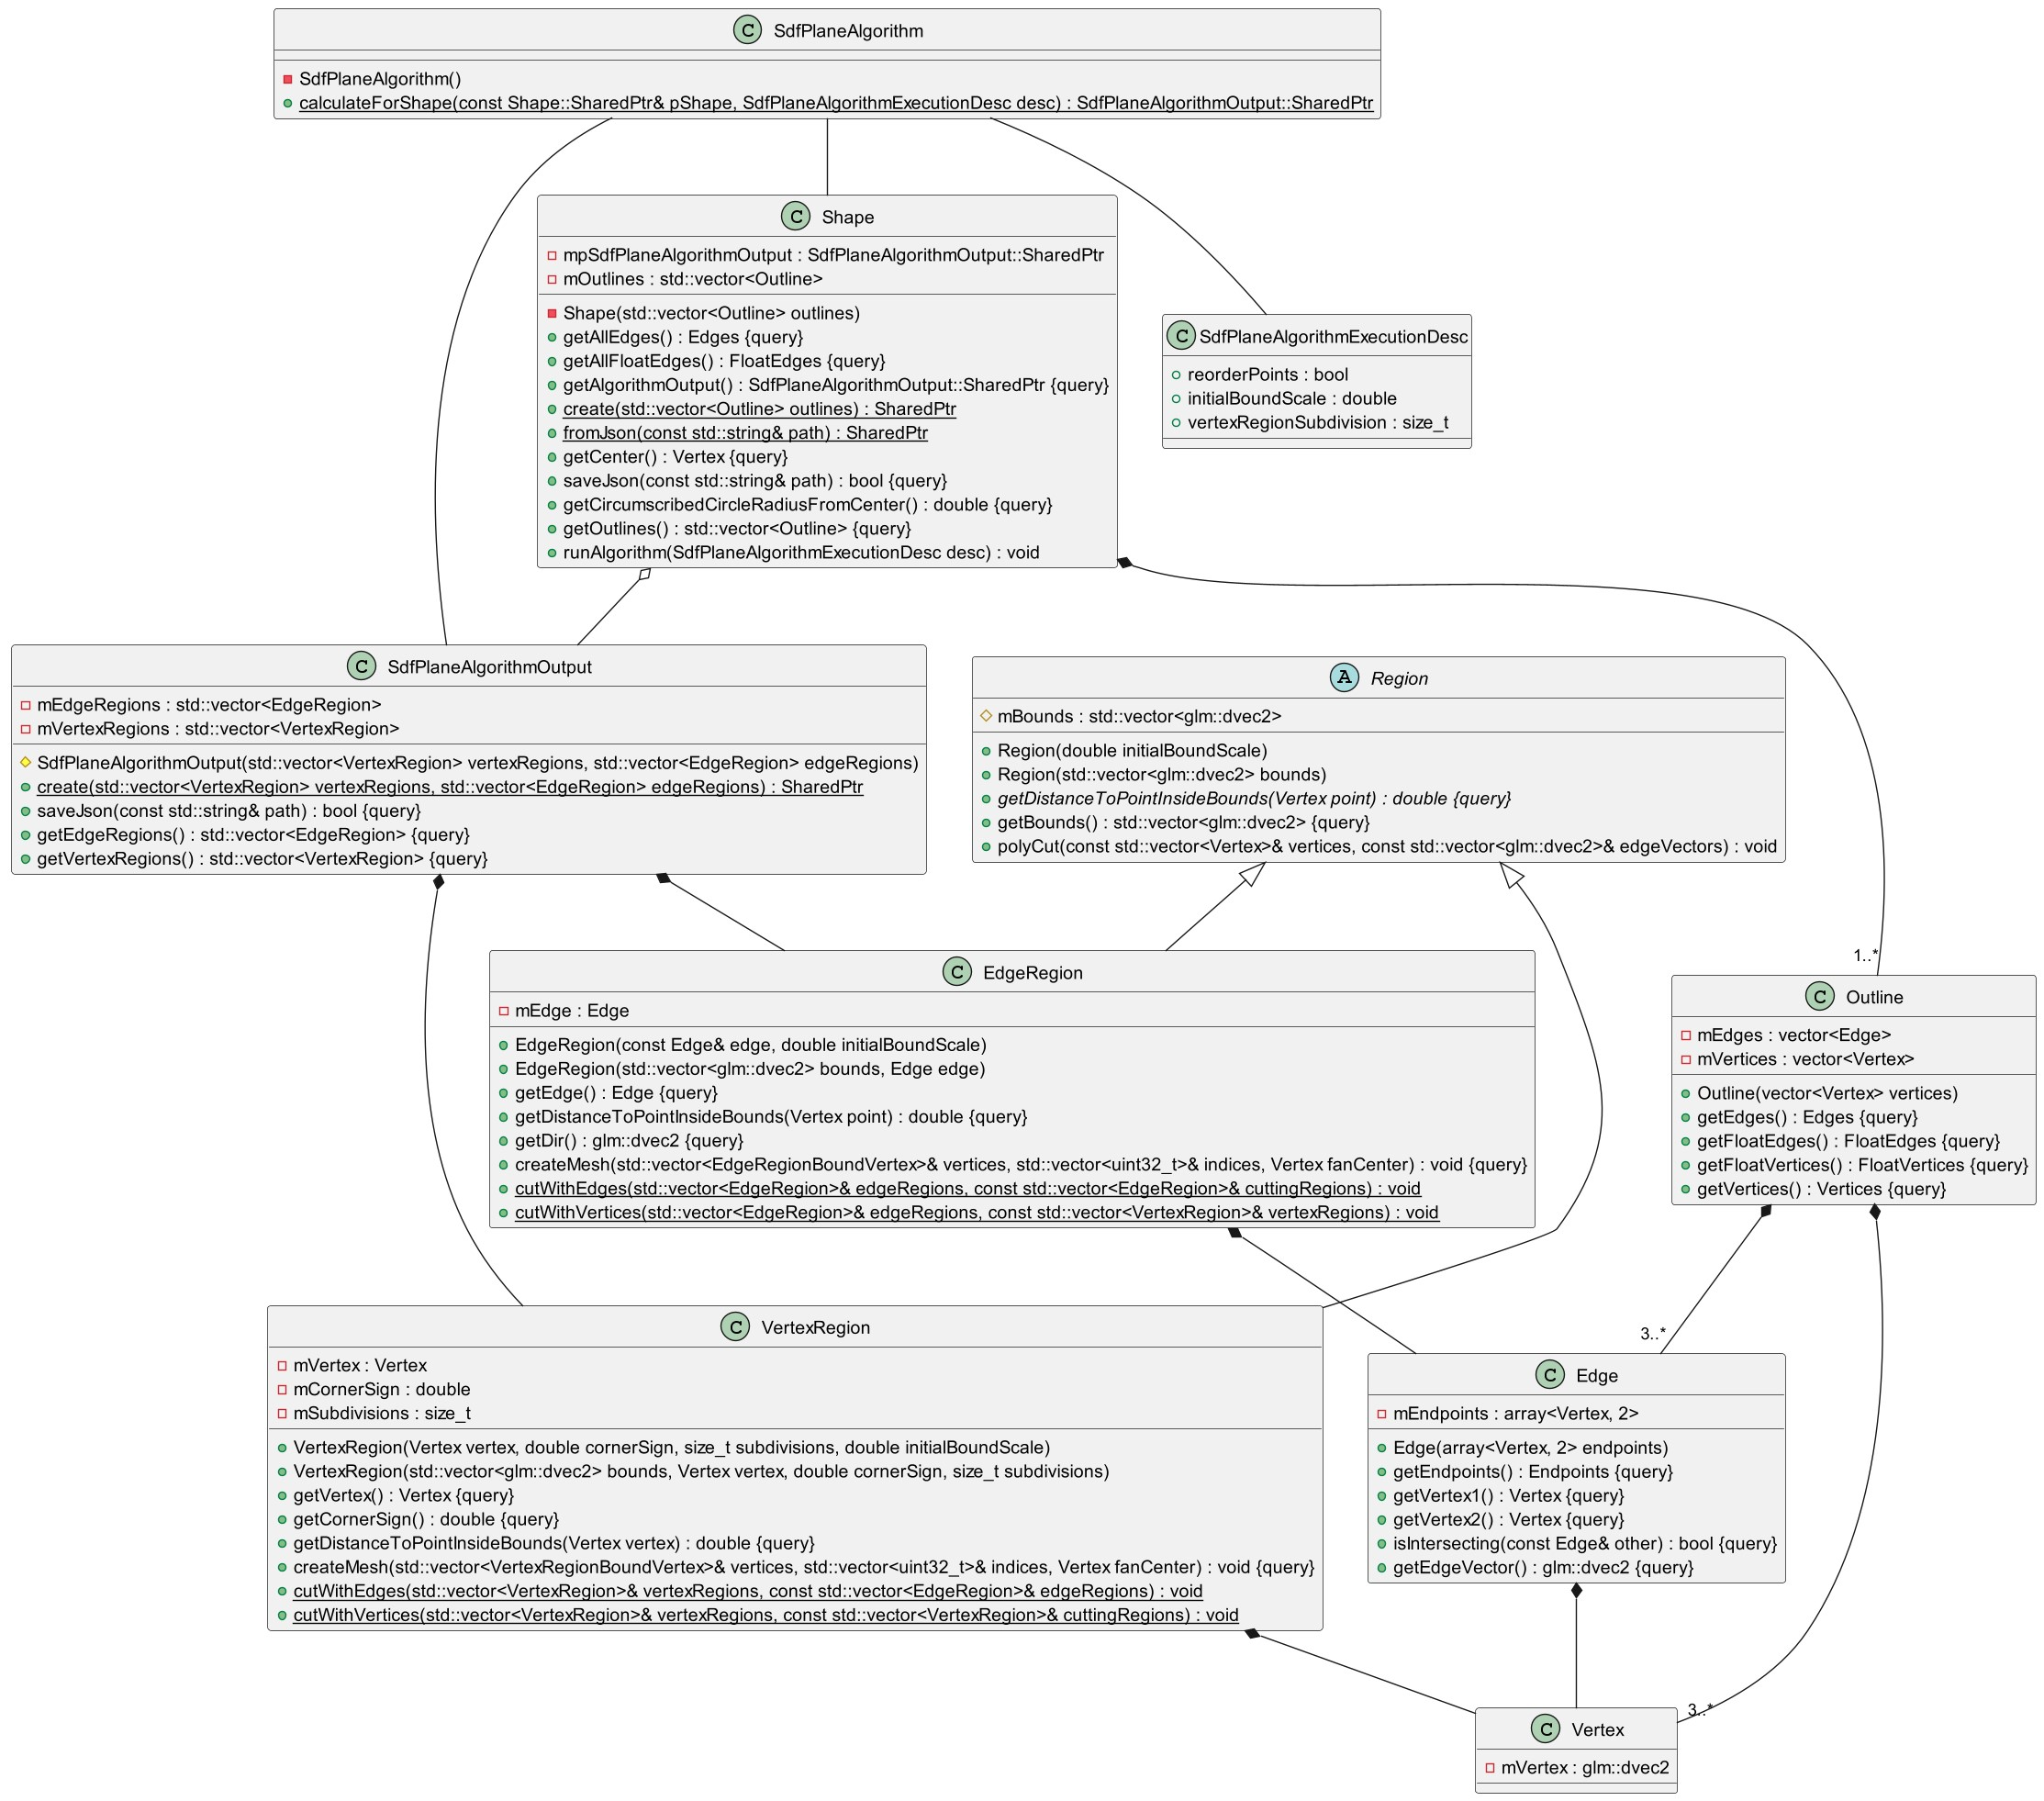
\includegraphics[width=1\linewidth]{images/class_algorithm.png}
    \caption{Az algoritmus osztálydiagramja}
    \label{fig:class_algorithm-1}
\end{figure}

\subsection{A régiók meghatározása}

A régiók vágása több lépésen keresztül történik, először felhasználjuk az információt ami az adott régió eleméhez tartozik. Csúcspontok esetén a két szomszédos él normálvektora mentén ejtünk egy-egy vágást. Élek esetében pedig a normálvektor mentén a két végponton kívül eső részt vágjuk le.

\begin{figure}[H]
    \centering
    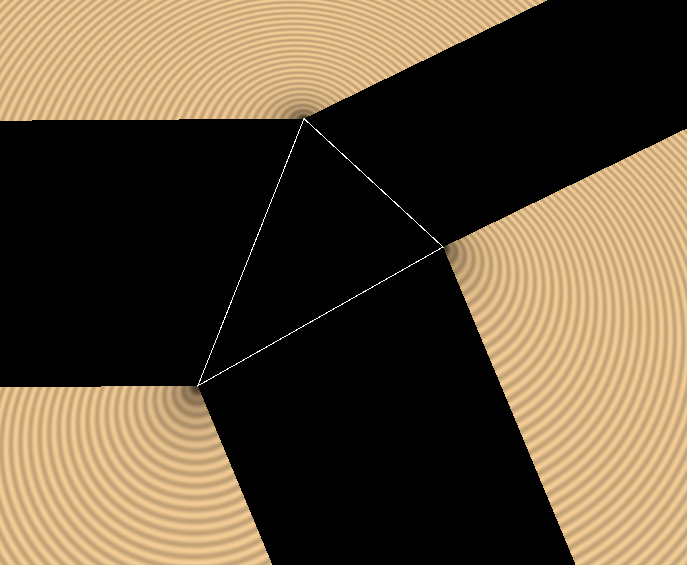
\includegraphics[width=.6\linewidth]{images/initial_vertex_regions.png}
    \caption{Csúcs régiók kezdeti határai}
    \label{fig:initial_vertex_regions-1}
\end{figure}

\begin{figure}[H]
    \centering
    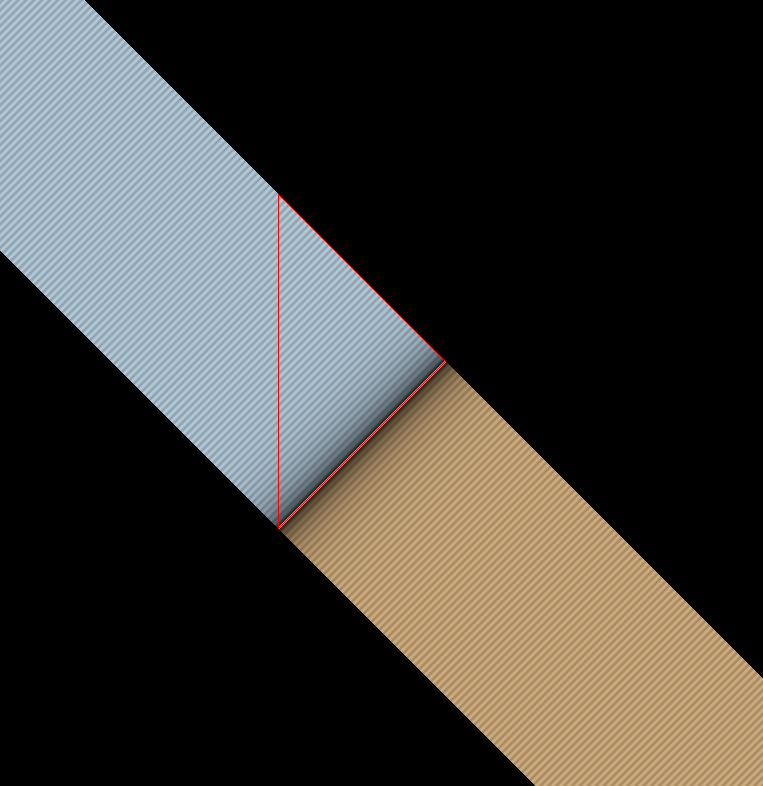
\includegraphics[width=.6\linewidth]{images/initial_segment_regions.png}
    \caption{él régiók kezdeti határai}
    \label{fig:initial_segment_regions-1}
\end{figure}

Az algoritmus következő lépéseként minden régiót elvágunk az összes többi régióhoz tartozó csúccsal és szakasszal. Eredményül a sokszög Voronoj-diagramja egy közelítését kapjuk, ahol a régiók között némi átfedés van. Ezt az átfedést a raszterizáció során a Z-puffer algoritmus oldja fel és jeleníti meg a megfelelő régiót.

\begin{figure}[H]
    \centering
    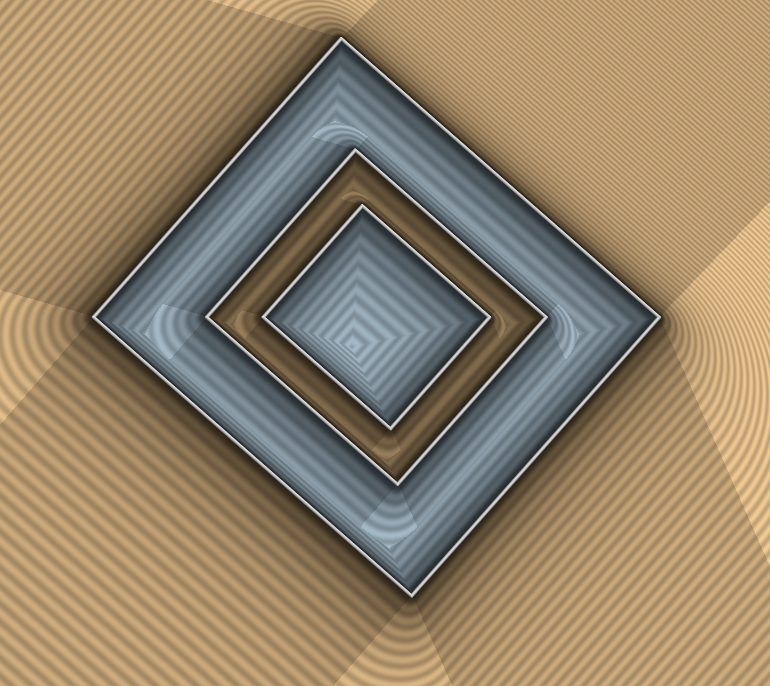
\includegraphics[width=.6\linewidth]{images/algorithm_output_top_down.png}
    \caption{Alakzat felülnézete}
    \label{fig:algorithm_output_top_down-1}
\end{figure}
\begin{figure}[H]
    \centering
    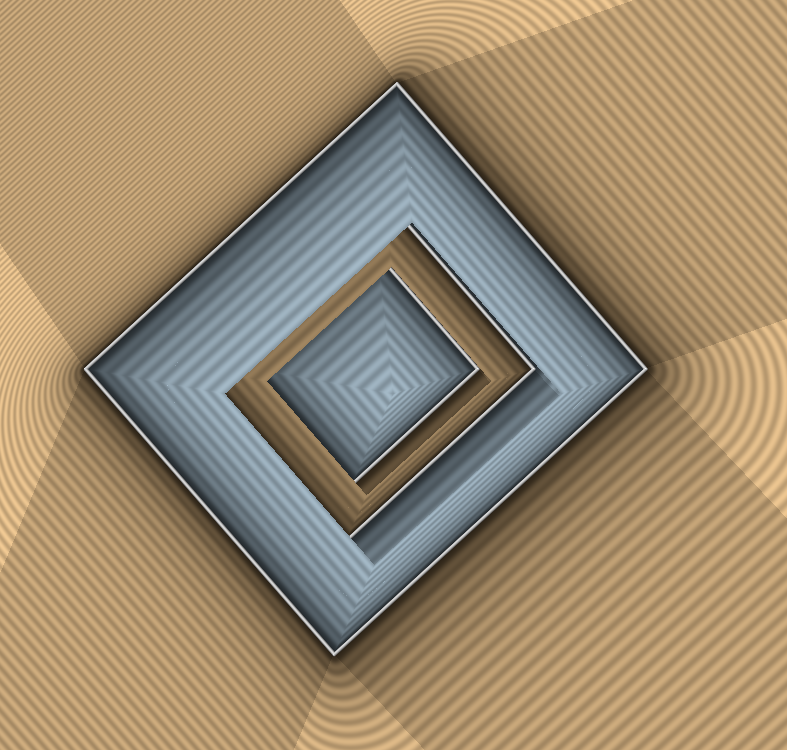
\includegraphics[width=.6\linewidth]{images/algorithm_output_bottom_up.png}
    \caption{Alakzat alulnézetből}
    \label{fig:algorithm_output_bottom_up-1}
\end{figure}

\subsection{Z-puffer algoritmus (Mélységi teszt)}
A mélységi teszt egy módszer a raszterizálásban arra, hogy eldöntsük, hogy az egymást átfedő geometriák közül melyik kerüljön megjelenítésre. Az algoritmus a GPU-n hajtódik végre és úgy működik, hogy rajzoláskor nem csak a képernyő színpufferébe ír, hanem egy másodlagos pufferbe (mélységi puffer), ahol számon tartja, hogy minden egyes elemhez a színpufferben milyen mélység tartozik. Az alkalmazás esetében színpufferbe csak akkor írunk, ha az új szín mélysége alacsonyabb (közelebb van a kamerához) a mélységi pufferben tárolt jelenlegi értéknél.

\subsection{Csúcs - csúcs vágások}

Azok a pontok, amelyek két pont között egyenlő távolságra helyezkednek el kollineárisak. Ebben a lépésben meghatározzuk azt az egyenest és annak a mentén végzünk egy vágást. Ez a művelet nem hagy átfedést a régióhatárok között. A \ref{fig:vertex_vertex_cut-1}-ös ábrán láthatjuk a vágás eredményést.

\iffalse
Legyen \textit{a} pont a régióhoz tartozó csúcs és \textit{b} pont a sokszög egy pontja, ami segítségével a vágást szeretnénk végrehajtani \textit{V} régión. A vágás algoritmusa a következő:

\begin{algorithm}[H]
    \caption{csúcs - csúcs vágás}
    \label{alg:vertex_cut_vertex}
    \textbf{Bemenet:} A régió határait definiáló sokszög csúcspontjai \textit{V} és \textit{a}, \textit{b} csúcspontok
    \textbf{Kimenet:} A régió új határai \textit{V}'
    \begin{algorithmic}[1]
        \State $e = b - a$ \Comment{A vágás egyenesére merőleges normálvektor.}
        \If{$||e|| <= \epsilon$}
            \State \textbf{return} V \Comment{Ha a két csúcs egybeesik, akkor nem végzünk módosítást.}
        \Else
            \State $m = (a + b) * 0.5$ \Comment{Meghatározzuk a két csúcs közötti pontot.}
            \State \textbf{return} polyCut($V$, $m$, $e$) \Comment{$V$ konvex poligont elvágjuk $m$ pont és $e$ normálvektor által meghatározott egyenes mentén.}
        \EndIf
    \end{algorithmic}
\end{algorithm}
\fi

\begin{figure}[H]
    \centering
    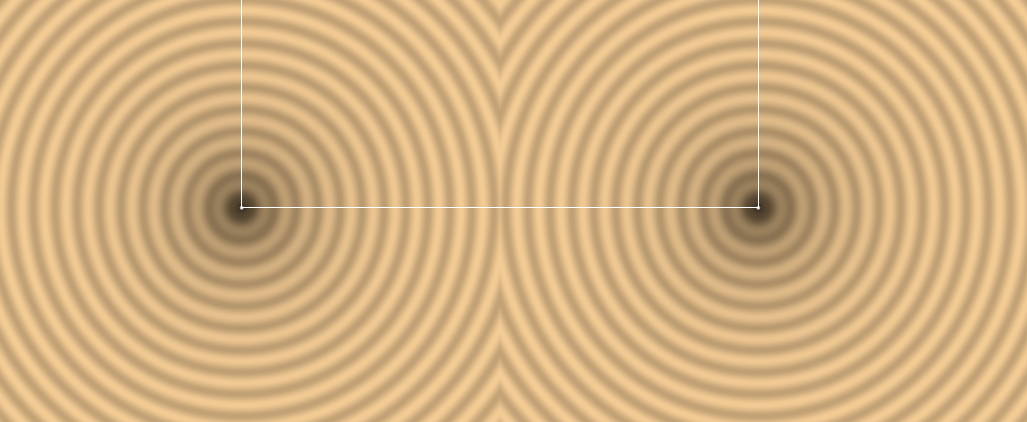
\includegraphics[width=1\linewidth]{images/vertex_vertex_cut.png}
    \caption{Csúcs - csúcs vágás eredménye}
    \label{fig:vertex_vertex_cut-1}
\end{figure}

\subsection{csúcs - él vágás} \label{vertex_segment_cut}
Azok a pontok, amelyek egy ponttól és egy egyenestől azonos távolságra vannak, egy parabolán helyezkednek el, ahol a parabola fókuszpontja megegyezik a vágási régióhoz tartozó csúccsal. Ebben a lépésben konstans számú vágást hajtunk végre a parabola görbéje mentén a csúcs régión. Minél nagyobb a vágások száma, annál pontosabb közelítést kapunk a csúcs régió Voronoj-cellájához. A \ref{fig:vertex_segment_cut-1}-os ábrán láthatjuk a vágás eredményést.

\begin{figure}[H]
    \centering
    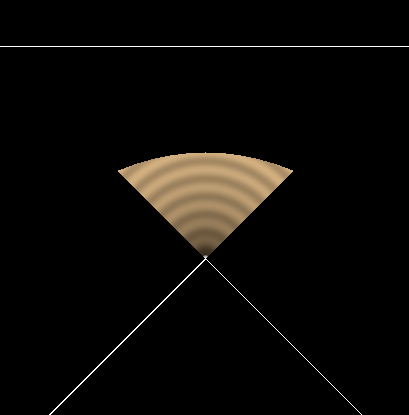
\includegraphics[width=.55\linewidth]{images/vertex_segment_cut.png}
    \caption{csúcs - él vágás eredménye}
    \label{fig:vertex_segment_cut-1}
\end{figure}

\subsection{Él - csúcs vágás}
Az él és csúcs közötti Voronok-cella határ a csúcs oldaláról konvex, az él oldaláról egy konkáv tartományt eredményez. A \ref{vertex_segment_cut}-es szekcióban meghatároztuk a parabolát, ami a csúcshoz tartozik. A számítások leegyszerűsítése érdekében az él esetében csak egy egyenes mentén vágunk úgy, hogy a csúcs régió paraboláját lefedjük, majd raszterizáláskor a Z-puffer algoritmus segítségével kerül feloldásra az átfedés. A lépés eredménye a \ref{fig:segment_vertex_cut-1}-es ábrán látható.

\begin{figure}[H]
    \centering
    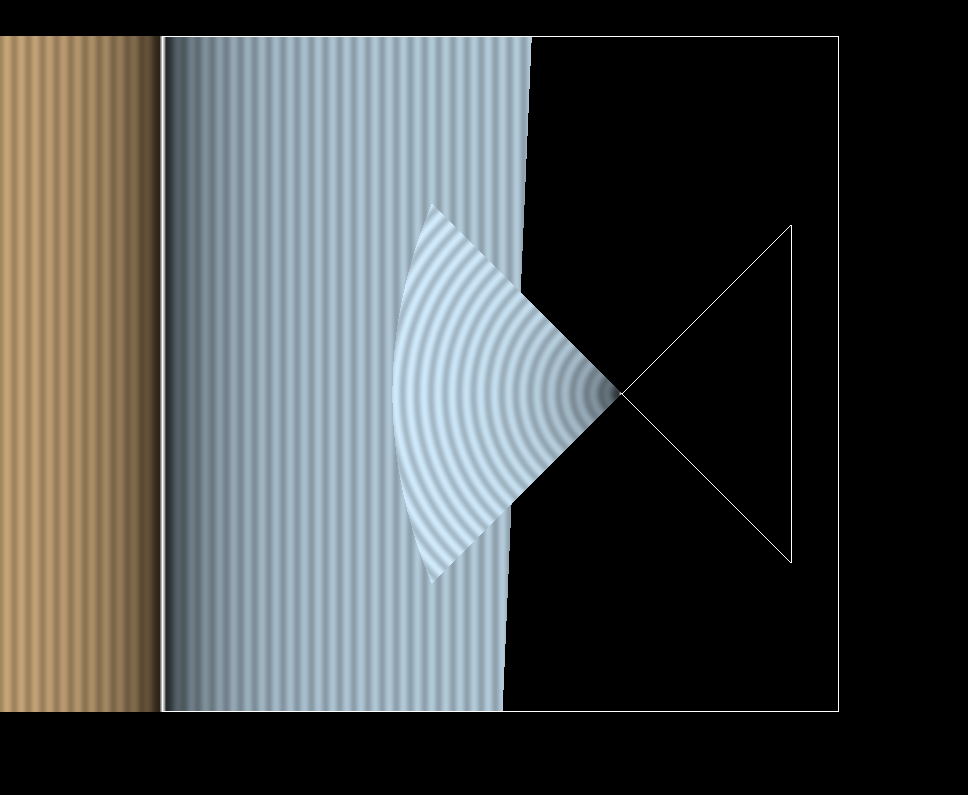
\includegraphics[width=.55\linewidth]{images/segment_vertex_cut.png}
    \caption{Él - csúcs vágás eredménye}
    \label{fig:segment_vertex_cut-1}
\end{figure}

\subsection{Él - él vágás}
Él - él vágás esetén figyelembe kell vennünk azoknak relatív pozícióját. Két él közötti rész három tartományra osztható fel: Az a tartomány, ahol az élek belső tartománya vannak közelebb egymáshoz, itt egy egyenes menén helyezkednek el az egyenlő távolságra lévő pontok, és két olyan tartomány, ahol az egyik élhez tartozó csúcshoz vagyunk közelebb, ahol a határ parabolikus. Ebben a lépésben egyetlen egyenes mentén vágunk élenként, az egyenesből és két parabolából álló összetett görbét lefedve. A vágással átfedések keletkeznek, amit a Z-puffer algoritmus old fel. A lépés eredménye a \ref{fig:segment_segment_cut-1}-as ábrán látható.

\begin{figure}[H]
    \centering
    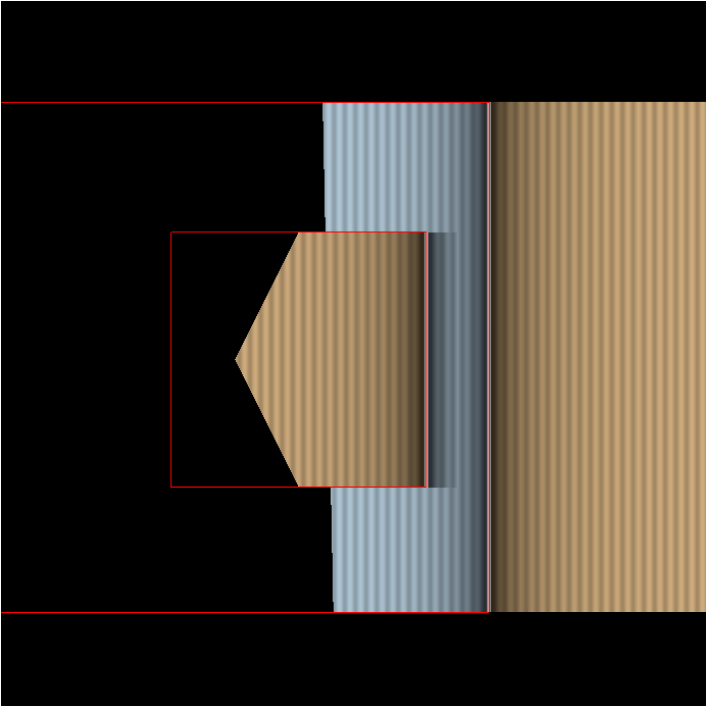
\includegraphics[width=.55\linewidth]{images/segment_segment_cut.png}
    \caption{Él - él vágás eredménye}
    \label{fig:segment_segment_cut-1}
\end{figure}

\section{A szerkesztő megtervezése}
A szerkesztő alapját az Autodesk Maya ,,construction history" funckiója inspirálta. Maya-ban a szerkesztett objektum az elvégzett műveletek sorozatából tevődik össze, ha egy köztes műveletet megváltoztatunk, akkor lehetőségünk van a rákövetkező műveleteket újra végrehajtani, közben egy teljesen eltérő eredményt kapva.

Az alkalmazásban, amit készítettem az alakzatunkat állapot átmenetekkel módosíthatjuk, ahol minden változtatáskor egy állapottal bővül a szerkesztő verme. A verem adatstruktúra természetéből adódóan a visszalépés triviális triviális művelet, mivel csak el kell vetnünk a verem tetejéről a módosítást. Az alkalmazásban a teljesítményre való tekintettel a veremben az átmenet által készített új állapot is tárolásra kerül, így minimalizálva a potenciálisan nagy számításigényű műveletek túlzott számban való kiértékelését. \textit{Megjegyzés: A jelenlegi implementáció nem támogatja az előrelépés és a köztes műveletek módosítását.}

A szerkesztő tervezésében különös figyelmet kapott annak skálázhatósága bővíthetőség szempontjából.
